\section{Architettura Back-End} \label{sec:archback}

Coerentemente alla struttura imposta dall'adozione di una Clean Architecture, il back-end dell'applicazione è organizzato tramite delle classi controller, use case, repository e data source.\\
Per collegare l'interfaccia grafica lato front-end con il funzionamento dell'applicativo lato back-end, sono state implementate delle server actions per chiamare i controller relativi all'azione desiderata.\\
I controller eseguono la chiamata allo use case relativo, che costituisce ed implementa la business logic dell'intero sistema.\\
Per accedere alle fonti dei dati, necessari a realizzare le funzionalità definite dai casi d'uso, le classi use cases si relazionano con delle classi repositories, nelle quali è posta la logica di persistenza, che presentano i metodi per lettura, scrittura ed eliminazione dei dati.\\
La singola classe repository si interfaccia alla classe data source ad essa associata, la quale presenta i metodi che intervengono concretamente sulle fonti dei dati per compiere le funzioni richieste sui database.\\
Una volta terminate le operazioni nel data source, il controllo torna alla repository, la quale ritorna i dati recuperati allo use case quando richiesto. Completata la funzionalità definita dal caso d'uso, il flusso di controllo torna al controller che dovrà gestire la risposta verso la server action da cui tutto è iniziato.

\begin{figure}[h!]
    \centering  
    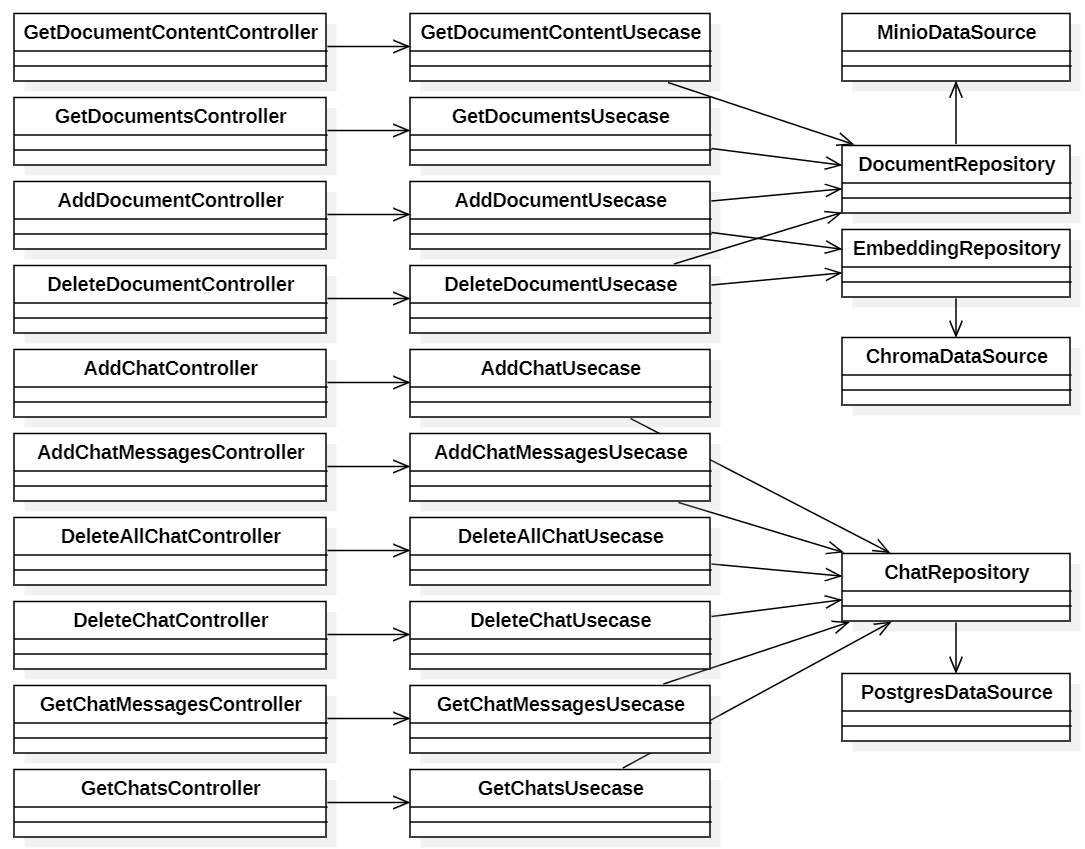
\includegraphics[width=0.7\textwidth]{backendview.png}
    \caption{UML introduttivo delle classi del back-end}
\end{figure}

\newpage


\subsection{Server Actions} \label{subsec:serveractions}

\subsubsection{addDocument}
\textbf{Parametri}
\begin{itemize}
    \item \textit{data: FormData}.
\end{itemize}
\textbf{Descrizione}\\
Questa funzione asincrona lato server effettua una chiamata a AddDocumentController, passando il parametro data. Data contiene una \textit{string} model e un \textit{File} file, che rappresentano il modello che deve presentare il nuovo documento e il file da aggiungere. Gestisce l'aggiunta di un documento inviando i dati al controller e si occupa di gestire eventuali errori che si possono verificano durante il processo.


\subsubsection{deleteDocument}
\textbf{Parametri}
\begin{itemize}[itemsep=-4pt]
    \item \textit{name: string};
    \item \textit{model: IModel}.
\end{itemize}
\textbf{Descrizione}\\
Questa funzione asincrona lato server effettua una chiamata a DeleteDocumentController, passando i parametri name e model, che rappresentano il nome del documento da eliminare e il modello che non deve più presentare tale documento. Gestisce l'eliminazione di un documento inviando i dati al controller e si occupa di gestire eventuali errori che si possono verificano durante il processo.

\subsubsection{getDocument}
\textbf{Parametri}
\begin{itemize}
    \item \textit{model: IModel}.
\end{itemize}
\textbf{Descrizione}\\
Questa funzione asincrona lato server effettua una chiamata a GetDocumentsController, passando il parametro model, che rappresenta il modello da cui prendere i documenti associati. Gestisce il recupero delle informazioni dei documenti inviando i dati al controller e si occupa di gestire eventuali errori che si possono verificano durante il processo.

\subsubsection{getDocumentContent}
\textbf{Parametri}
\begin{itemize}[itemsep=-4pt]
    \item \textit{docName: string};
    \item \textit{model: IModel}.
\end{itemize}
\textbf{Descrizione}\\
Questa funzione asincrona lato server effettua una chiamata a GetDocumentContentController, passando i parametri docName e model, che rappresentano il nome del documento da cui recuperare il link per la visualizzazione e il modello che presenta tale documento. Gestisce il recupero dell'informazione inviando i dati al controller e si occupa di gestire eventuali errori che si possono verificano durante il processo.

\subsubsection{addChat}
\textbf{Parametri}
\begin{itemize}
    \item \textit{title: string}.
\end{itemize}
\textbf{Descrizione}\\
Questa funzione asincrona lato server effettua una chiamata a AddChatController, passando il parametro title, che rappresenta il nome della sessione di conversazione da aggiungere. Gestisce la creazione della sessione inviando i dati al controller e si occupa di gestire eventuali errori che si possono verificano durante il processo.

\subsubsection{addChatMessages}
\textbf{Parametri}
\begin{itemize}
    \item \textit{messages: ICustomMessages}.
\end{itemize}
\textbf{Descrizione}\\
Questa funzione asincrona lato server effettua una chiamata a AddChatMessagesController, passando il parametro messages, che rappresenta il messaggio da salvare relativo ad una sessione di conversazione. Gestisce il salvataggio del messaggio inviando il dato al controller e si occupa di gestire eventuali errori che si possono verificano durante il processo.

\subsubsection{deleteAllChat}
\textbf{Descrizione}\\
Questa funzione asincrona lato server effettua una chiamata a DeleteAllChatController, passando la string che rappresenta la query per eliminare tutti i dati relativi a sessioni e chat history. Gestisce l'eliminazione di queste informazioni inviando il dato al controller e si occupa di gestire eventuali errori che si possono verificano durante il processo.

\subsubsection{deleteChat}
\textbf{Parametri}
\begin{itemize}
    \item \textit{id: number}.
\end{itemize}
\textbf{Descrizione}\\
Questa funzione asincrona lato server effettua una chiamata a DeleteChatController, passando il parametro id, che rappresenta il valore univoco della sessione di conversazione da eliminare. Gestisce l'eliminazione della sessione inviando i dati al controller e si occupa di gestire eventuali errori che si possono verificano durante il processo.

\subsubsection{getChatMessages}
\textbf{Parametri}
\begin{itemize}
    \item \textit{id: number}.
\end{itemize}
\textbf{Descrizione}\\
Questa funzione asincrona lato server effettua una chiamata a GetChatMessagesController, passando il parametro id, che rappresenta il valore univoco della sessione di conversazione da cui recuperare la chat history. Gestisce il recupero dati della sessione inviando il parametro al controller e si occupa di gestire eventuali errori che si possono verificano durante il processo.

\subsubsection{getChats}
\textbf{Descrizione}\\
Questa funzione asincrona lato server effettua una chiamata a GetChatsController, con cui recupera le informazioni delle sessioni di conversazione attive nell'applicazione. Gestisce il recupero dati delle sessioni ed eventuali errori che si verificano durante il processo.

\newpage

\newpage
